\documentclass{beamer}

% for themes, etc.
\mode<presentation>
%\usetheme{Warsaw}
%\usecolortheme{dolphin}
%{\usetheme{Singapore}}
%{ \usetheme{lined} }
{\usetheme{Dresden}}
\usepackage{fontspec}   %加這個就可以設定字體
\usepackage{xeCJK}       %讓中英文字體分開設置
%\setCJKmainfont{標楷體} %設定中文為系統上的字型,而英文不去更動,使用原TeX字型
\XeTeXlinebreaklocale "zh"             %這兩行一定要加,中文才能自動換行
\XeTeXlinebreakskip = 0pt plus 1pt     %這兩行一定要加,中文才能自動換行

\usepackage{amsmath,amssymb,amsfonts,booktabs}
\usepackage{epic}
\usepackage{mathpazo}  % fonts are up to you
%\usepackage{astats,epsfig}
\usepackage{graphicx,epsfig,subfigure}
\usepackage{pdftexcmds}
\usepackage{xcolor}
\usepackage{amsthm}
\newtheorem{thm1}{Theorem 1.}
\newtheorem{thm2}{Theorem 2}
\newtheorem{lem1}{Lemma 1.}
\renewcommand{\proofname}{\ctxfk \textbf{Proof.}}
%\usepackage{array,booktabs}
% these will be used later in the title page
\title{Penalized Least Squares with LASSO and SCAD}
\author{San-Teng Huang,Shang-Chien Ho,Hsing-Cheng Pan}
\institute{National Dong Hwa University}
\date{2019/01/04}
\begin{document}
		\begin{frame}
		\titlepage
        \end{frame}
        
        \begin{frame}
		\frametitle{Outline} % make a frame titled "Outline"
		\tableofcontents % show TOC and highlight current section
        \end{frame}
\section{Introduction}
    \begin{frame}
\frametitle{Multiple Linear Regression}
	\emph{•}Consider multiple linear model: 
	\begin{equation}
		Y_i =  \beta_0 + \beta_1 X_{i1} +\beta_2 X_{i2} +...+\beta_{p-1} X_{ip-1}  + \varepsilon_i \quad , i=1,2,...,n
	\end{equation} 
	\\\quad where $\boldsymbol{\beta}$ is $p \times 1$ vector, $\mathbf{X}$ is $n \times p$ matrix,
	\\\quad and $\varepsilon_i \,\, i.i.d$ with mean $0$, variance $\sigma^2$, for $i=1,...,n$.
      \\\emph{•} Assume only some parameters are non-zero.   
      \\\quad the true $\boldsymbol{\beta_0}=(\beta_{01},\beta_{02},...,\beta_{0p})=(\boldsymbol{\beta_{01}^T},\boldsymbol{\beta_{02}^T})=(\boldsymbol{\beta_{01}^T},\boldsymbol{0})$    
    \end{frame}
    
    \begin{frame}
      \frametitle{Goal}
      \large\emph{•}Variable selection  
      \\\normalsize\quad the true $\boldsymbol{\beta_0}=(\beta_{01},\beta_{02},...,\beta_{0p})=(\boldsymbol{\beta_{01}^T},\boldsymbol{\beta_{02}^T})=(\boldsymbol{\beta_{01}^T},\boldsymbol{0})$
    \end{frame}
         
\section{LASSO }     
\begin{frame}
\frametitle{The LASSO\hspace{1mm}: $\ell_1$ penalty }  
\emph{•}Tibshirani\hspace{1mm}(1996) introduced the LASSO\hspace{0.5mm}:\hspace{0.5mm}least absolute
\\\quad shrinkage and selection operator.
\\\emph{•}LASSO coefficients are the solutions to the $\ell_1$ optimization
\\\quad problem :
\\\begin{equation}
\quad\quad\, \min\limits_{\boldsymbol{\beta}}\sum_{i=1}^n(y_i-\sum_{j=1}^px_{ij}\beta_j)^2 \quad s.t.\, ||\beta||_1\leq{t}
\end{equation} 
%\\\emph{•}This is equivalent to :
\\\begin{equation}
\Leftrightarrow \min\limits_{\boldsymbol{\beta}}\sum_{i=1}^n(y_i-\sum_{j=1}^px_{ij}\beta_j)^2+\lambda\sum_{j=1}^p|\beta_j|
\end{equation} 
\quad where $||\beta||_1 = \sum_{j=1}^p|\beta_j|$
\end{frame}

\begin{frame}
\frametitle{$\lambda$(or $t$) as a tuning parameter}
%\emph{•}Note that,\hspace{0.5mm}we have a tuning parameter $\lambda$ to control the 
%\\\quad amount of regularization.%Regularization:維持現有的features,但降低部分不重要feature的影響力。這對於有著許多feature的hypothesis很有幫助。
\emph{•}The constraint :
\\\begin{equation*}
\sum_{j=1}^p|\beta_j|\leq{t} \quad or \quad \lambda\sum_{j=1}^p|\beta_j|
\end{equation*}
%\\\qquad\emph{•}Hence,\hspace{0.5mm}have a "path" of solutions indexed by t.
\\\qquad\emph{•}If $\lambda=0$, then it means no shrinkage.
\\\qquad\quad (hence is the OLS solutions.)
\\\qquad\emph{•}Large enough $\lambda$ (or small enough $t$) will set some coefficients
\\\qquad\quad exactly equal to 0.

\end{frame}

\begin{frame}
\emph{•} Ridge regression's coefficients are the solutions to the $\ell_2$
\\\quad optimization problem :
\\\begin{equation*}
\quad\quad\quad \min\limits_{\boldsymbol{\beta}}\sum_{i=1}^n(y_i-\sum_{j=1}^px_{ij}\beta_j)^2 \quad s.t.\, ||\beta||_2\leq{t}
\end{equation*} 
\\\begin{equation*}
\Leftrightarrow \min\limits_{\boldsymbol{\beta}}\sum_{i=1}^n(y_i-\sum_{j=1}^px_{ij}\beta_j)^2+\lambda\sum_{j=1}^p\beta_j^2
\end{equation*}
\quad where $||\beta||_2 =\sqrt{ \sum_{j=1}^p\beta_j^2}$
\end{frame}

\begin{frame}
\frametitle{Why the LASSO set coefficients exactly equal to 0 ? }
\begin{figure}[h]
\begin{center}
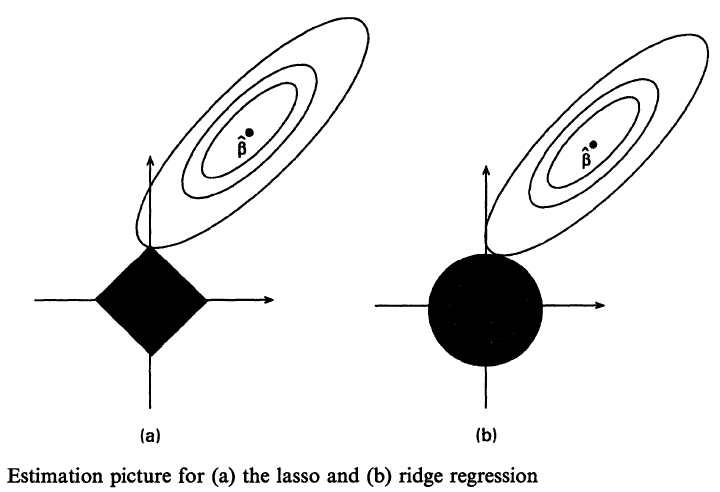
\includegraphics[width=8.3cm]{image06}
\end{center}
\end{figure}
\end{frame}



\begin{frame}
\frametitle{}
\begin{figure}[h]
	\begin{center}
		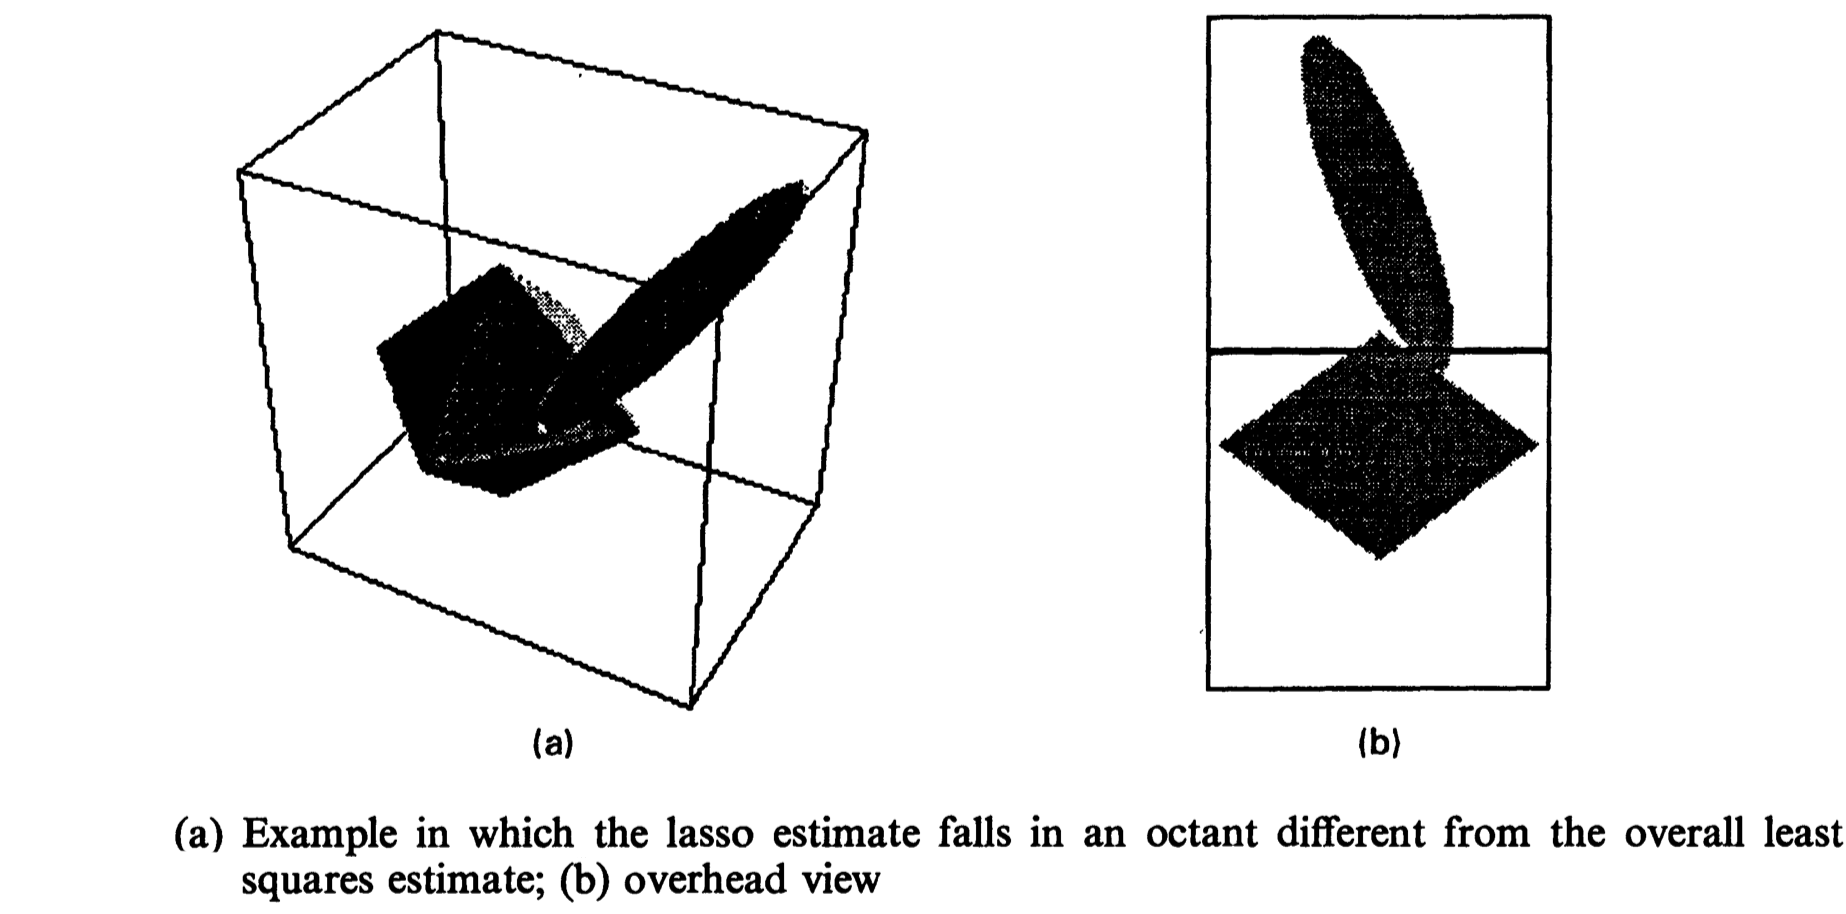
\includegraphics[width=8.3cm]{3_dimension}
	\end{center}
\end{figure}
\end{frame}
%%%%%%%%%%%%%%%%%%%%%%%%%%%%%%%%%%%%%%%%%%%%%%%%%%%%%

\begin{frame}
\frametitle{Example}
\emph{•}Consider model: 
\begin{equation*}
Y_i =  \beta_1 X_{i1} +\beta_2 X_{i2} +...+\beta_{10} X_{i10}  + \varepsilon_i \quad , i=1,2,...,100
\end{equation*} 
\\\quad where $\mathbf{X} \sim MVN(0 ,\Sigma)$, $\Sigma$ be covariance matrix with 
\\\quad for $j , k = 1,...,10,\, j \neq k,$ $Var(X_j) = 1,$ $Cov(X_j,X_k) = 0.5 $ 
\\\quad and $\varepsilon_i \sim N(0,3^2), \,i=1,...,100$.
\\\quad the true $\boldsymbol{\beta_0}=(3 , 1.5 , 2 , -7 , 15 ,0 ,0 , 0 , 0 ,0)$    
\\\emph{•} With 100 replication, count the number of estimated value 
\\\quad greater than $10^{-3}$. The parameter $\lambda$ choosed by 10-fold cross
\\\quad validation.  

\end{frame}

\begin{frame}
\fontsize{9pt}{13pt}
\begin{tabular}[t]{|l|c|c|c|c|}
	\hline
	            & OLS       &       & LASSO($\lambda = 0.2636$)      & \\  
	\hline
                & bias(sd)    & count(\%) & bias(sd)     & count(\%) \\
	\hline  
	$\beta_1=3$ & 0.0400(0.44)&    1  & -0.1529(0.42)  & 1\\
	$\beta_2=1.5$ &0.0307(0.45) & 1     &-0.1655(0.42)   & 1\\
	$\beta_3=2$ & 0.0474(0.43) & 1     &-0.1435(0.42)   &1\\
	$\beta_4=7$ &-0.0495(0.40) & 1     &0.3294(0.39)  &1\\
	$\beta_5=15$&0.0623(0.47) & 1      &-0.1395(0.45)  &1\\
	$\beta_6=0$&-0.0102(0.45) & 1     &0.0272(0.25)  &0.59\\ 
	$\beta_7=0$&0.0028(0.39) & 0.99 	  &0.0547(0.22)  &0.54\\     	                  
	$\beta_8=0$&-0.0636(0.43) & 1 	  &0.0215(0.25)  &0.55\\
	$\beta_9=0$&0.0180(0.44) & 1 	  &0.0744(0.25)  &0.61\\
	$\beta_{10}=0$&-0.0678(0.39) & 1 	  &0.0045(0.21)  &0.58\\
	
	\hline
\end{tabular}
\end{frame}     

%%%%%%%%%%%%%%%%%%%%%%%%%%%%%%%%%%%%%%%%%%%%%%%%%%%%% 
\section{SCAD}     
    \begin{frame}
      \frametitle{Penalized Least Squares}
      \emph{•}To minimize
      \begin{equation}
         Q(\boldsymbol{\beta})=\sum_{i=1}^{n}(y_i-\sum_{j=1}^px_{ij}\beta_j )^2 + n\sum_{j=1}^p p_{\lambda}(|\beta_j|)
      \end{equation}
      where $p_{\lambda}(|\beta|)$ is a penalty function.
      \\\emph{•}The penalized least squares estimator is
      \begin{equation*}
         \hat{\boldsymbol{\beta}} = arg \min\limits_{\boldsymbol{\beta}} Q(\boldsymbol{\beta}) 
      \end{equation*}
    \end{frame}
    
    \begin{frame}
      \frametitle{Penalty function}
      \emph{•}LASSO($L_1$-penalty):
      \begin{equation*}
          p_{\lambda}(|\beta|)=\lambda|\beta|
      \end{equation*}
      \\\emph{•}Smoothly Clipped Absolute Deviation (SCAD):
      \begin{equation*}
           p_{\lambda}(|\beta|)=\begin{cases} \lambda|\beta| \hspace{3cm},|\beta|\leq\lambda \\
                                       -(\dfrac{|\beta|^2-2a\lambda|\beta|+\lambda^2}{2(a-1)}) ,\lambda<|\beta|\leq a\lambda \\
                                \dfrac{(a+1)\lambda^2}{2} \hspace{2.1cm},|\beta|>a\lambda          \end{cases}    
      \end{equation*} 
      \quad where $a=3.7$ 
    \end{frame}
    
    \begin{frame}
     \frametitle{Plot of $p_{\lambda}(|\beta|)$:}
      \begin{figure}[h]
      \begin{center}
      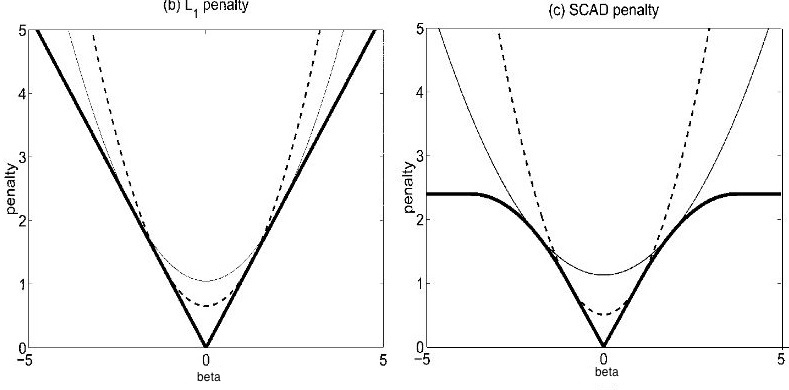
\includegraphics[width=10cm]{image01}
      \end{center}
      \end{figure}
    \end{frame}
    
    \begin{frame}
    \frametitle{What is good penalty function?}
    \emph{•}{\bf{Unbiasedness}}: The estimator is nearly unbiased when the true 
    \\\quad unknown parameter is large to avoid modeling bias.
    \\\emph{•}{\bf{Sparsity}}: The estimator is a thresholding rule, which sets small
    \\\quad estimated coefficients to zero.
    \\\emph{•}{\bf{Continuity}}: The estimator is continuous in data $\boldsymbol{x}$ to avoid
    \\\quad instability in model prediction. 
\end{frame}
    
    \begin{frame}
      \begin{tabular}[t]{|l|c|c|c|}
	\hline
	                                & Unbiasedness  & Sparsity & Continuity \\
	 \hline  
	$L_1$-penalty(LASSO)               & no            & yes      & yes \\
	$L_2$-penalty(ridge regression)    & no            & no       & yes \\      
	 SCAD                           & yes           & yes      & yes \\
	 \hline
	  \end{tabular}
    \end{frame}
\section{Simulation}
%%%%%%%%%%%%%%%%%%%%%%%%%%%%%%%%%%%%%%%%%%%%%%%%%%%%%%%%%%
\begin{frame}
\frametitle{Conti. Example}
\emph{•}Consider model: 
\begin{equation*}
Y_i =  \beta_1 X_{i1} +\beta_2 X_{i2} +...+\beta_{10} X_{i10}  + \varepsilon_i \quad , i=1,2,...,100
\end{equation*} 
\\\quad where $\mathbf{X} \sim MVN(0 ,\Sigma)$, $\Sigma$ be covariance matrix with 
\\\quad for $j , k = 1,...,10,\, j \neq k,$ $Var(X_j) = 1,$ $Cov(X_j,X_k) = 0.5 $ 
\\\quad and $\varepsilon_i \sim N(0,3^2), \,i=1,...,100$.
\\\quad the true $\boldsymbol{\beta_0}=(3 , 1.5 , 2 , -7 , 15 ,0 ,0 , 0 , 0 ,0)$    
\\\emph{•} With 100 replication, count the number of estimated value 
\\\quad greater than $10^{-3}$. The parameter $\lambda$ choosed by 10-fold cross
\\\quad validation.  

\end{frame}

\begin{frame}
\fontsize{7.5pt}{12pt}
\begin{tabular}[t]{|l|c|c|c|c|}
	\hline
	& SCAD($\lambda = 0.3792$)       &       & LASSO($\lambda = 0.2636$)      & \\  
	\hline
	& bias(sd)    & count(\%) & bias(sd)     & count(\%) \\
	\hline  
	$\beta_1=3$ & 0.0415(0.42)&    1  & -0.1529(0.42)  & 1\\
	$\beta_2=1.5$ &-0.0394(0.52) & 1     &-0.1655(0.42)   & 1\\
	$\beta_3=2$ & 0.0390(0.43) & 1     &-0.1435(0.42)   &1\\
	$\beta_4=7$ &-0.0571(0.38) & 1     &0.3294(0.39)  &1\\
	$\beta_5=15$&0.0740(0.46) & 1      &-0.1395(0.45)  &1\\
	$\beta_6=0$&-0.0230(0.23) & 0.46     &0.0272(0.25)  &0.59\\ 
	$\beta_7=0$&0.0053(0.17) & 0.36 	  &0.0547(0.22)  &0.54\\     	                  
	$\beta_8=0$&-0.0303(0.21) & 0.44	  &0.0215(0.25)  &0.55\\
	$\beta_9=0$&0.0218(0.19) & 0.48 	  &0.0744(0.25)  &0.61\\
	$\beta_{10}=0$&-0.0279(0.16) & 0.39 	  &0.0045(0.21)  &0.58\\
	
	\hline
\end{tabular}
\end{frame}     

\begin{frame}
\fontsize{10pt}{14pt}
\begin{tabular}[t]{|l|c|c|c|c|}
	\hline
                     	& SCAD       &       & LASSO      & \\  
	\hline
	$\lambda=0.3792$ & bias(sd)    & count(\%) & bias(sd)     & count(\%) \\
	\hline  
	$\beta_1=3$ & 0.0415(0.42)&    1  & -0.2232(0.42)  & 1\\
	$\beta_2=1.5$ &-0.0394(0.52) & 1     &-0.2341(0.41)   & 1\\
	$\beta_3=2$ & 0.0390(0.43) & 1     &-0.2100(0.42)   &1\\
	$\beta_4=7$ &-0.0571(0.38) & 1     &0.5049(0.39)  &1\\
	$\beta_5=15$&0.0740(0.46) & 1      &-0.2126(0.45)  &1\\
	$\beta_6=0$&-0.0230(0.23) & 0.46     &0.0420(0.19)  &0.47\\ 
	$\beta_7=0$&0.0053(0.17) & 0.36 	  &0.0578(0.18)  &0.42\\     	                  
	$\beta_8=0$&-0.0303(0.21) & 0.44 	  &0.0317(0.20)  &0.43\\
	$\beta_9=0$&0.0218(0.19) & 0.48 	  &0.0802(0.20)  &0.41\\
	$\beta_{10}=0$&-0.0279(0.16) & 0.39 	  &0.0175(0.15)  &0.39\\

	\hline
\end{tabular}
\end{frame}     
    
\begin{frame}
\fontsize{10pt}{14pt}
\begin{tabular}[t]{|l|c|c|c|c|}
	\hline
	& SCAD       &       & LASSO      & \\  
	\hline
	$\lambda=0.7585$ & bias(sd)    & count(\%) & bias(sd)     & count(\%) \\
	\hline  
	$\beta_1=3$ & 0.1655(0.50)&   1  & -0.4177(0.44)  & 1\\
	$\beta_2=1.5$ &-0.4698(0.57) & 0.97     &-0.4319(0.42)   & 1\\
	$\beta_3=2$ &-0.2262(0.64) & 1     &-0.4000(0.44)   &1\\
	$\beta_4=7$ &0.0947(0.38) & 1     &1.1121(0.40)  &1\\
	$\beta_5=15$&0.2376(0.46) & 1      &-0.4214(0.46)  &1\\
	$\beta_6=0$&0.0018(0.05) & 0.18     &0.0357(0.10)  &0.26\\ 
	$\beta_7=0$&0.0148(0.06) & 0.14 	  &0.0462(0.12)  &0.23\\     	                  
	$\beta_8=0$&0.0083(0.06) & 0.12 	  &0.0396(0.12)  &0.19\\
	$\beta_9=0$&0.0186(0.07) & 0.15 	  &0.0616(0.15)  &0.27\\
	$\beta_{10}=0$&0.0035(0.04) & 0.09 	  &0.0163(0.07)  &0.18\\
	
	\hline
\end{tabular}
\end{frame}         

\section{Conclusion}

\begin{frame}
\frametitle{Conclusion}
\emph{•} Variable selection via penalized least squares.
\begin{tabular}[t]{|l|c|c|c|}
	\hline
	& Unbiasedness  & Sparsity & Continuity \\
	\hline  
	$L_1$-penalty(LASSO)               & no            & yes      & yes \\
	$L_2$-penalty(ridge regression)    & no            & no       & yes \\      
	SCAD                           & yes           & yes      & yes \\
	\hline
\end{tabular}
\end{frame}

\end{document}        